%%%%%%%%%%%%%%%%%%%%%%%%%%%%%%%%%%%%%%%%%%%%%%%%%%%%%%%%%%%%%%%%%%%%%%%%%%%%%%%%%%%%%%%%%%%%%%%%%%%
%%%%%%%%%%%%%%%%%%%%%%%%%%%%%%%%%%%%%%%%%%%%%%%%%%%%%%%%%%%%%%%%%%%%%%%%%%%%%%%%%%%%%%%%%%%%%%%%%%%
\section{Conceptos, fisiolog\'ia}

En esta secci\'on se exponen conceptos propios de la biolog\'ia y que ayudar\'an a definir
al sujeto de estudio: registros de PSG en adultos mayores con y sin PDC.
Se pretende que la exposici\'on sea accesible a\'un sin una preparaci\'on 
especializada en fisiolog\'ia, especialmente considerando que el autor pertenece a tal grupo.

%%%%%%%%%%%%%%%%%%%%%%%%%%%%%%%%%%%%%%%%%%%%%%%%%%%%%%%%%%%%%%%%%%%%%%%%%%%%%%%%%%%%%%%%%%%%%%%%%%%

\subsection{Adulto mayor}

Se define como adulto mayor a un individuo de 60 a\~nos o m\'as que habite un pa\'is en v\'ias de
desarrollo, o 65 a\~nos en pa\'ises desarrollados \cite{Hita14}.
En esta etapa 
%ocurren cambios fisiol\'ogicos, psicol\'ogicos y sociales
el organismo sufre cambios fisiolo\'ogicos y psicol\'ogicos que dificultan la capacidad de
adaptaci\'on al ambiente, teniendo como consecuencia una mayor suceptibilidad a padecer enfermedades
y morir en consecuencia \cite{Hita14}.


%El envejecimiento es un proceso biológico que se caracteriza por la disminución de las funciones 
%que hacen más susceptible al ser humano de padecer enfermedades y morir a consecuencia de 
%ellas [1]. 
%Durante esta etapa ocurren cambios biol\'ogicos, psicol\'ogicos y sociales, normales e 
%inherentes a todo individuo debido a que el organismo va perdiendo la habilidad para responder 
%ante el estr\'es y mantener la regulación homeost\'atica y metabólica, teniendo como consecuencia 
%la disminuci\'on de las capacidades cognitivas y de sobrevivencia, reflejándose en la imposibilidad 
%de adaptarse a situaciones de restricci\'on o sobrecarga de cualquier tipo [4,9,10]

El envejecimiento considerado normal viene determinado por una serie de procesos moleculares, 
celulares, fisiol\'ogicos y psicol\'ogicos que conducen directamente al deterioro de funciones 
cognitivas, específicamente en la atenci\'on y memoria \cite{Navarrete03,Park09}.
%Aunque el envejecimiento es un proceso normal, la 
La
funcionalidad durante la vejez no es homog\'enea
en general; se relaciona con el estilo de vida, los factores de riesgo, el acceso a la
educaci\'on y las acciones de promoci\'on a la salud realizadas en edades m\'as tempranas
\cite{Ohayon04,Sanhueza14}.

%A pesar de ser un proceso natural, no todos los individuos envejecen de la misma forma debido a 
%que la calidad de vida y funcionalidad durante la vejez est\'a relacionada con los aprendizajes 
%adquiridos durante la infancia, adolescencia y edad adulta \cite{Ohayon04}. 
%Los estilos de vida, los factores de riesgo, la accesibilidad a la educaci\'on y la promoci\'on 
%de la salud adoptados a lo largo de la vida son fundamentales al momento de llegar a esta etapa 
%para que en el presente de esta se logre autonom\'ia, a pesar de la edad y los padecimientos que 
%se tengan \cite{Sanhueza14}.

%%%%%%%%%%%%%%%%%%%%%%%%%%%%%%%%%%%%%%%%%%%%%%%%%%%%%%%%%%%%%%%%%%%%%%%%%%%%%%%%%%%%%%%%%%%%%%%%%%%

%\subsubsection{Cambios en la anatom\'ia cerebral con la vejez}

En un principio se consideraba que el envejecimiento cerebral ocurr\'ia fundamentalmente por una 
muerte neuronal programada \cite{Coleman87}, sin embargo, estudios realizados con tejido cerebral 
post mortem de adultos mayores que en vida fueron sanos, mostraron que dicha muerte neuronal no 
alcanza un 10\% en su totalidad \cite{Esiri07}. 
En este sentido, los cambios morfol\'gicos que 
sufren las neuronas durante el envejecimiento son abundantes, observ\'andose una importante 
disminuci\'on de la arborizaci\'n dendr\'itica as\'i como en la densidad y volumen \cite{Hita14}. 
%La disminución en la arborización dendr\'itica y de las espinas dendr\'iticas de las neuronas 
%piramidales de la corteza prefrontal, temporal superior, pre central y occipital \cite{Hita14}. 
%Dichas alteraciones morfol\'ogicas conducen durante el envejecimiento a una disminuci\'on de 
%la densidad sin\'aptica y a una desmielinizaci\'on ax\'onica en neuronas de la 
%neocorteza \cite{Terry}.
Con el paso del tiempo, la organizaci\'on an\'atomo-funcional del cerebro sufre modificaciones 
que traen como consecuencia la afectaci\'on de diferentes capacidades cognitivas, 
sin embargo, 
la vulnerabilidad de los circuitos neuronales ante los procesos que ocurren durante el 
envejecimiento no suceden de forma homog\'enea en todo el cerebro \cite{Hita14}.

%Por otro lado, la relevancia del estudio de los cambios anat\'omicos asociados al envejecimiento 
%fisiol\'ogico ha ido aumentando al permitir evaluar como dichos cambios se correlacionan con 
%el deterioro funcional y cognitivo que caracteriza a las personas mayores, facilita la 
%identificaci\'on de estadios tempranos de diferentes patolog\'ias neurodegenerativas estableciendo 
%diferencias entre estas y los cambios asociados al envejecimiento fisiol\'ogico \cite{Hita14}.

%%%%%%%%%%%%%%%%%%%%%%%%%%%%%%%%%%%%%%%%%%%%%%%%%%%%%%%%%%%%%%%%%%%%%%%%%%%%%%%%%%%%%%%%%%%%%%%%%%%

\subsection{El sue\~no}

%(Esta secci\'on tambi\'en es copiada, por el momento)

El sue\~no se define como ''un proceso vital c\'iclico complejo y activo, compuesto por varias 
fases y que posee una estructura interna caracter\'istica, con diversas interrelaciones en los 
sistemas hormonales y nerviosos'' \cite{FernandezConde07}. 
%Una suspensi\'on f\'acilmente reversible 
%de la interacci\'on sensoriomotriz con el medio ambiente, por lo general asociados con el 
%dec\'ubito y la inmovilidad.
El sue\~no en el ser humano se puede caracterizar por las siguientes propiedades\cite{CarrilloMora}
%Las caracter\'isticas conductuales que se asocian con el sue\~no en el ser humano pueden 
%enumerarse de la siguiente forma\cite{CarrilloMora} 
\begin{enumerate}
\item Disminuci\'on de conciencia y reactividad a est\'imulos externos
\item F\'acilmente reversible\footnote{Lo cual lo diferencia de otros estados 
patol\'ogicos como el estupor y el coma}
\item Inmovilidad y relajaci\'on muscular
\item Periodicidad t\'ipica circadiana (diaria)
\item Los individuos adquieren una postura estereotipada
\item La privaci\'on induce alteraciones conductuales y 
fisiol\'ogicas, adem\'as de que genera una ''deuda'' acumulativa
\end{enumerate}

%%%%%%%%%%%%%%%%%%%%%%%%%%%%%%%%%%%%%%%%%%%%%%%%%%%%%%%%%%%%%%%%%%%%%%%%%%%%%%%%%%%%%%%%%%%%%%%%%%%

%El sustrato neurol\'ogico relacionado con la ritmicidad del sueño se encuentra en el hipot\'alamo, 
%estructura que tiene diversidad de conexiones en el Sistema Nervioso Central, con el fin de 
%ejercer una funci\'on o funciones capaces de sincronizar el organismo 
%\cite{FernandezConde07,Cabrera14}.
%Las estructuras l\'imbicas, tales como la am\'igdala y el hipot\'alamo, tambi\'en estar\'ian 
%activadas, lo que explicar\'ia los fen\'omenos emotivos durante la fase de sue\~no REM ya que 
%las emociones est\'an directamente vinculadas con estas zonas cerebrales \cite{Bonet08}.

%%%%%%%%%%%%%%%%%%%%%%%%%%%%%%%%%%%%%%%%%%%%%%%%%%%%%%%%%%%%%%%%%%%%%%%%%%%%%%%%%%%%%%%%%%%%%%%%%%%
%%%%%%%%%%%%%%%%%%%%%%%%%%%%%%%%%%%%%%%%%%%%%%%%%%%%%%%%%%%%%%%%%%%%%%%%%%%%%%%%%%%%%%%%%%%%%%%%%%%

\subsection{Electroencefalograma}

%Esta secci\'on est\'a fuermente basada\footnote{A este punto, ya
%no es una copia, pero quiz\'a ser\'ia mejor diversificar las fuentes} 
%en el cap\'itulo de libro 
%''The origin of biopotentials'' de John William Clark \cite{clark98}.

La actividad el\'ectrica en el cerebro de animales ya hab\'ia sido descrita desde finales del
siglo XIX, pero se le atribuye al psiquiatra alem\'an Hans Berger ser el primero en analizar
este fen\'omeno sistem\'aticamente adem\'as de acu\~nar el t\'ermino ''electroencefalograma'' (EEG)
para referirse a las fluctuaciones en los potenciales de acci\'on registradas en el cerebro.
De manera convencional, la actividad el\'ectrica del cerebro 
se registra en tres locaciones diferentes: en la corteza cerebral
expuesta (electrocorticograma, ECoG), a trav\'es de agujas incrustadas en el tejido nervioso
(registro profundo), o el cuero cabelludo (EEG).

%La actividad el\'ectrica en el cerebro de animales con y sin anestesia ya hab\'ia sido descrito
%cualitativamente desde el siglo XIX, pero el primero en analizarla sistem\'aticamente fue el
%psiquiatra alem\'an Hans Berger, quien introdujo el t\'ermino electroencefalograma (EEG) para
%denotar las fluctuaciones en los potenciales registrados en el cerebro. [tengo citas sobre ello]
%De manera convencional, la actividad el\'ectrica del cerebro se registra usando tres tipos de
%electrodos: 'scalp', cortical y electrodos de profundidad.
%Cuando los electrodos se colocan en la superficie expuesta del cerebro (cortex) el
%registro se llama electrocorticograma (ECoG). Tambi\'en se pueden usar electrodos de aguja
%aislada fina --de varios dise\~nos-- incrustados en el tejido nervioso del cerebro, en
%cuyo caso el registro se conoce como 'registro profundo'. Seg\'un se reporta, el da\~no al
%tejido cerebral es sorprendentemente peque\~no si se usan agujas con un tama\~no
%y dise\~no adecuados.

As\'i la actividad el\'ectrica cerebral se mida
en el cuero cabelludo, la corteza cerebral o las profundidades 
del mismo,
las fluctuaciones de potenciales registrados representan una superposici\'on
de potenciales de campo producidos por una amplia variedad de 
generadores de corriente dentro de un medio conductor volum\'etrico --es decir, los elementos
neuronales activos generan, cada cual, corrientes que son conducidas y disipada a 
trav\'es del espacio.
A su vez, estos generadores de campos el\'ectricos corresponden a agregados de elementos
neuronales con interconexiones complejas: dendritas, somas y axones.
%M\'as a\'un, la arquitectura del tejido cerebral no es uniforme
%espacialmente.
A ello hay que adicionar que la arquitectura cerebral es altamente no homog\'enea.

%%%%%%%%%%%%%%%%%%%%%%%%%%%%%%%%%%%%%%%%%%%%%%%%%%%%%%%%%%%%%%%%%%%%%%%%%%%%%%%%%%%%%%%%%%%%%%%%%%%

%\subsubsection{Potenciales bioel\'ectricos del cerebro}

%Los registros unipolares de potencial en la superficie cortical, relativos a un potencial de
%referencia remoto, pueden ser vistos como una medida del potencial de campo integrado sobre la
%frontera de un volumen conductor 'grande' que contiene un conjunto de fuentes de potenciales de 
%campo.

%Bajo condiciones normales los potenciales de campo producidos por axones, en 
%la corteza cerebral, aportan muy poco al potencial registrado;
%%al potencial de superficie integrado; 
%esto d
Debido a que los axones en la corteza cerebral tienen orientaciones muy diversas --con
%orientaciones muy diversas 
respecto a la superficie-- y a que disparan de manera as\'incrona, el aporte neto de estos campos
al potencial registrado es negligible bajo condiciones normales.
%En consecuencia, su influencia neta sobre el potencial de campo en la superficie es negligible.
Una excepci\'on, muy importante, ocurre en caso de una respuesta evocada por un est\'imulo
simult\'aneo (s\'incronizado) del del n\'ucleo 
tal\'amico o de las aferentes nerviosas.
%, que se proyecta en el cortex v\'ia axones corticotal\'amicos).
Estas respuestas sincronizadas suelen tener una amplitud relativamente alta, y
son referidas como 'potenciales evocados'.
%, y su amplitud es
%relativamente alta.

%%%%%%%%%%%%%%%%%%%%%%%%%%%%%%%%%%%%%%%%%%%%%%%%%%%%%%%%%%%%%%%%%%%%%%%%%%%%%%%%%%%%%%%%%%%%%%%%%%%

\subsubsection{EEG cl\'inico}

El sistema m\'as usado para la colocaci\'on de los electrodos en el EEG con fines cl\'inicos es el 
'International Federation 10--20 system' \cite{Jasper58,AASM07} mostrado en la figura \ref{img1020}. 
Este sistema usa varios
referentes anat\'omicos estandarizados para la ubicaci\'on de los electrodos.

La representaci\'on de los canales de EEG es referida como un \textbf{montaje}
En un montaje bipolar, cada canal mide la diferencia entre dos electrodos adyacentes.
En un monntaje referencial, cada canal mide la diferencia entre un electrodo y un electrodo
de referencia, usualmente la oreja.
%\footnote{Existen otros tipos de montaje, como el promedio (promedio sobre electrodos adyacentes,
%como los sistemas 5\% y 10\%) o el Laplaciano (parecido al promedio, pero usando un filtrado
%basado en pesos relacionados con la distancia entre electrodos)
%. S\'olo hablo del referencial
%y diferencial porque uno se usa en el estudio y otro es importante hist\'oricamente.}
Aunque los mismos eventos el\'ectricos se registran en cada uno de los montajes,
aparecen en un diferente formato seg\'un el caso. Los potenciales cambiantes
son amplificados por amplificadores diferenciales acoplados de alta ganancia.
La se\~nal resultante es grabada y graficada.

\begin{figure}
\centering
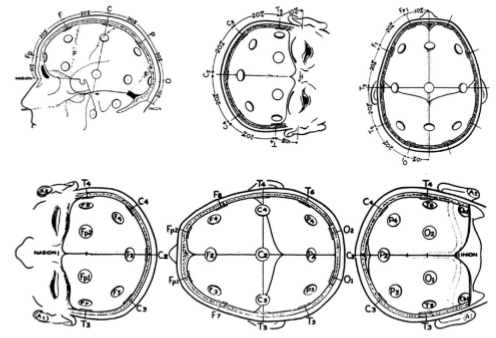
\includegraphics[width=0.8\linewidth]{figura_6.png} 
\caption{El sistema 10--20, recomendado por la
International Federation of EEG Societies. 
%\cite{Jasper58,AASM07}
}
\label{img1020}
\end{figure}

%The system most often used to place electrodes for monitoring the clinical
%EEG is the International Federation 10–20 system shown in Figure 4.28. This
%system uses certain anatomical landmarks to standardize placement of EEG
%electrodes. The representation of the EEG channels is referred to as a
%montage. 
%In the bipolar montage, each channel measures the difference
%between two adjacent electrodes. 
%In the referential montage, each channel
%measures the diffference between one electrode and a reference electrode,
%such as on the ear. In the average reference montage, each channel measures
%the difference between one electrode and the average of all other electrodes.
%In the Laplacian montage, each channel measures the difference between one
%electrode and a weighted average of the surrounding electrodes. The differ-
%ential amplifier requires a separate ground electrode plus differential inputs to
%the electrode connections. The advantage of using a differential recording
%between closely spaced electrodes (between successive pairs in the standard
%system, for example) is cancellation of far-field activity common to both
%electrodes; one thereby obtains sharp localization of the response. 
%Although
%the same electric events are recorded in each of the ways, they appear in a
%different format in each case. The potential changes that occur are amplified by
%high-gain, differential, capacitively coupled amplifiers. The output signals are
%recorded and displayed.

En el EEG cl\'inico de rutina, los electrodos 
%son un problema: 
deben ser peque\~nos, deben estar
fijados al cuero cabelludo de manera sencilla con una distorsi\'on m\'inima debido al cuero cabelludo,
deben ser c\'omodos, y deben permanecer en el mismo sitio por largos periodos de tiempo.
El [encargado del registro] prepara la superficie del cuero cabelludo 
desengrasando el \'area de registro
limpi\'andola con alcohol, aplica una pasta conductora, pega los electrodos no-polarizables (Ag/AgCl)
al cuero cabelludo con pegamento (coloid\'on), y los sostiene en el sitio con cintas de caucho
--o se usa una gorra de caucho que contiene todos los electrodos.

%In the routine recording of clinical EEGs, the input electrodes are a
%problem. They must be small, they must be easily affixed to the scalp with
%minimal disturbance of the hair, they must cause no discomfort, and they must
%remain in place for extended periods of time. Technicians prepare the surface
%of the scalp, degrease the recording area by cleaning it with alcohol, apply a
%conducting paste, and glue nonpolarizable Ag/AgCl electrodes to the scalp
%with a glue (collodion) and hold them in place with rubber straps, or use a
%rubber cap that contains all electrodes.

El EEG usualmente se registra con el sujeto despierto pero relajado, descansando en una cama con 
los ojos cerrados; la posici\'on debe ser tal que los artefactos debidos al movimiento de 
electrodos en el 'scalp' sean m\'inimas. 
La actividad muscular, de la cara, cuello, orejas, etc., es quiz\'a la forma m\'as sutil de 
contaminaci\'on de los registros de EEG cuando se busca actividad espont\'anea del cerebro
durante una actividad, o la actividad evocada por est\'imulos sensoriales.
Por ejemplo, el espectro de frecuencias del potencial de campo producido por m\'usculos faciales
medianamente contra\'idos, incluye componentes de frecuencia que bien cuadran en el rango
usual del EEG (0.5--100 Hz).
Una vez se ha conseguido el estado de reposo en un adulto normal, sus registros de scalp
muestran un ritmo alfa dominante en el \'area parietal-occipital, mientras que en \'area
frontal ha un ritmo beta con baja amplitud y alta frecuencia --adem\'as del ritmo alfa.
En un sujeto normal hay cierta simetr\'ia entre los registros de los hemisferios derecho e 
izquierdo. 
La variedad de artefactos conocidos es muy basta.

%The EEG is usually recorded with the subject awake but resting recumbent
%on a bed with eyes closed. With the patient relaxed in such a manner, artifacts
%from electrode-lead movement are significantly reduced, as are contaminating
%signals from the scalp. 
%Muscle activity from the face, neck, ears, and so on is
%perhaps the most subtle contaminant of EEG records in the recording of both
%spontaneous ongoing activity in the brain and activity evoked by a sensory
%stimulus (evoked response). 
%For example, the frequency spectrum of the field
%produced by mildly contracted facial muscles contains frequency components
%well within the nominal EEG range (0.5 to 100 Hz). After technicians have
%achieved resting, quiescent conditions in the normal adult subject, the subject’s
%scalp recordings show a dominant alpha rhythm in the parietal-occipital areas,
%whereas in the frontal areas, there is a low-amplitude, higher-frequency beta
%rhythm in addition to the alpha rhythm. In the normal subject there is
%symmetry between the recordings of the right and left hemispheres. There
%can be a wide range of EEG measurement artifacts.

En general hay una relaci\'on entre el grado de actividad cerebral
y la 'frecuencia promedio' del EEG: la frecuancia incrementa progresivamente cuando hay altos
grados de actividad. Por ejemplo, las ondas delta se encuentran frecuentemente durante el
estupor, anestesia quir\'urgica, y sue\~no; las ondas theta son comunes en infantes;
las ondas alfa ocurren en estado de relajaci\'on; las ondas beta aparecen durante actividad
mental intensa.
Sin embargo, durante periodos de actividad mental las ondas se vuelven m\'as as\'incronas
que sincronizadas, de modo que la magnitud del potencial integrado de superficie
decrece a pesar de la alta actividad cortical.

%In general there is a relationship between the degree of cerebral activity
%and the average frequency of the EEG rhythm: The frequency increases
%progressively with higher and higher degrees of activity. For example, delta
%waves are frequently found in stupor, surgical anesthesia, and sleep; theta
%waves in infants; alpha waves during relaxed states; and beta waves during
%intense mental activity. However, during periods of mental activity, the waves
%usually become asynchronous rather than synchronous, so that the magnitude
%of the summed surface potential recording decreases despite increased cortical
%activity.

%%%%%%%%%%%%%%%%%%%%%%%%%%%%%%%%%%%%%%%%%%%%%%%%%%%%%%%%%%%%%%%%%%%%%%%%%%%%%%%%%%%%%%%%%%%%%%%%%%%

\subsection{Ritmos de sue\~no en el EEG}

Los registros de EEG desde el cuero cabelludo muestran una actividad el\'ectrica oscilatoria 
continua y cambiante. Tanto la intensidad como los patrones de esta actividad est\'an determinados
por los eventos de excitaci\'on conjunta del cerebro, resultante de las funciones en el
sistema reticular de activaci\'on del tallo cerebral \cite{Clark98}.
Estas 'ondas' observadas en los registros de potenciales el\'ectricos en el cerebro 
(\ref{ritmos}) son referidas como
\textbf{ondas cerebrales}, mientras que %el registro \textit{per se} recibe el nombre de EEG.

La frecuencia de las ondas cerebrales var\'ia entre 0.5 y 100 Hz, 
se ha identificado que su composici\'on est\'a fuertemente
relacionada con el grado de actividad cerebral, habiendo --por ejemplo-- diferencias claras
entre registros durante vigilia y sue\~no.
Aunque la mayor parte del tiempo el EEG es irregul y no muestra patrones claros,
es relativamente com\'un que muestre ondas cerebrales relativamente organizadas; para su estudio,
estas se clasifican en cuatro grandes grupos: alfa, beta, gamma, delta.


\begin{figure}
\centering
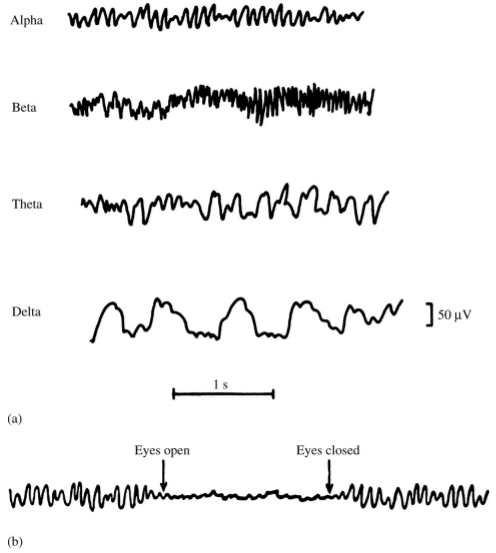
\includegraphics[width=0.7\linewidth]{figura_4.png} 
\caption{\textbf{(a)} Diferentes tipos de ondas normales en el EEG.
\textbf{(b)} Supresi\'on del ritmo alfa debido a una descarga dessincronizada cuando
el paciente abre los ojos.
%(From A. C. Guyton, Structure and Function of the Nervous System, 2nd ed.,
%Philadelphia: W.B. Saunders, 1972; used with permission.)
[Estos gr\'aficos ser\'an reconstruidos]
}
\label{ritmos}
\end{figure}


Las ondas alfa ocurren en frecuencias entre 8 y 13 Hz. 
Se encuentran en
los EEG --bajo condiciones normales--
de sujetos despiertos en un estado de quietud del pensamiento.
Estas ondas ocurren m\'as intensamente en la regi\'on occipital, pero tambi\'en pueden ser
registradas en las regiones frontal y parietal. Su voltaje aproximado est\'a entre 20 y 200 mV.
Cuando el sujeto duerme, las ondas alfa desaparecen completamente. 
Cuando el sujeto est\'a
despierto y su atenci\'on se dirige a una actividad mental espec\'ifica, las ondas alfa
son reemplaxadas por ondas dessincronizadas de mayor frecuencia y menor voltaje.
%En la figura \ref{ritmos} se muestra este efecto con la acci\'on de cerrar los ojos.

Las ondas beta ocurren en el rango de frecuencias de 14 a 30 Hz.
%, y usualmente
%--en especial durante actividad mental intensa-- hasta 50 Hz.
Normalmente se registran en las regiones parietal y frontal. A veces se les divide
 en dos tipos: beta I y beta II. Las ondas beta I tienen una frecuencia de cerca del doble a
 las ondas alfa, y son afectadas de manera similar por la actividad mental --desaparecen
y son reemplazadas por ondas dessincronizadas de menor amplitud.
Las ondas beta II, en cambio, aparecen durante una activaci\'on intensa del sistema nervioso
central y durante tensi\'on.

%Beta waves normally occur in the frequency range of 14 to 30 Hz, and
%sometimes—particularly during intense mental activity—as high as 50 Hz.
%These are most frequently recorded from the parietal and frontal regions of the
%scalp. They can be divided into two major types: beta I and beta II. The beta I
%waves have a frequency about twice that of the alpha waves. They are affected
%by mental activity in much the same way as the alpha waves (they disappear
%and in their place appears an asynchronous, low-voltage wave). The beta II
%waves, on the other hand, appear during intense activation of the central
%nervous system and during tension. Thus one type of beta activity is elicited by
%mental activity, whereas the other is inhibited by it.

Las ondas theta tienen frecuencias entre 4 y 7 Hz. Ocurren principalmente en las regiones
parietal y temporal en ni\~nos, pero pueden aparecer en algunos adultos durante 
estr\'es emocional, sobre todo durante periodos de decepsi\'on y frustraci\'on.
%Por ejemplo, pueden ser inducidos en el EEG de una persona frustrada una vez se le permite
%disfrutar una experiencia placentera, la cual es removida s\'ubitamente. Esto causa
%aproximadamente 20 s de ondas theta.

%Theta waves have frequencies between 4 and 7 Hz. These occur mainly in
%the parietal and temporal regions in children, but they also occur during
%emotional stress in some adults, particularly during periods of disappointment
%and frustration. For example, they can often be brought about in the EEG of a
%frustrated person by allowing the person to enjoy some pleasant experience
%and then suddenly removing the element of pleasure. This causes approxi-
%mately 20 s of theta waves.

Las ondas delta incluyen todas las ondas del EEG 'abajo de' 3.5 Hz. 
%A veces, estas ondas s\'olo
%aparecen cada 2 o 3 seg. 
Ocurren generalmente en el sue\~no profundo en infantes,
y despu\'es de enfermedades org\'anicas serias del cerebro.
Tambi\'en pueden ser registradas en cerebros de animales a los cuales se ha hecho 
transsecci\'on subcortical, produciendo una separaci\'on funcional entre la corteza
cerebral y el 
sistema reticular de activaci\'on del tallo cerebral. 
%Entonces, las ondas delta s\'olo pueden ocurrir en la cortreza cerebral,
%independientemente de la actividad en las regiones m\'as bajas del cerebro.

%%%%%%%%%%%%%%%%%%%%%%%%%%%%%%%%%%%%%%%%%%%%%%%%%%%%%%%%%%%%%%%%%%%%%%%%%%%%%%%%%%%%%%%%%%%%%%%%%%%

%\subsection{Patrones en el sue\~no}

%When an individual in a relaxed, inattentive state becomes drowsy and falls
%asleep, the alpha rhythm is replaced by slower, larger waves 
%(\ref{ritmosEEG},\cite{Jasper42}). 

En el sue\~no profundo se observan ondas delta muy irregulares. Junto con ellas, durante el sue\~no
medianamente profundo, ocurren trenes cortos de ondas parecidas a las alfa y que son referidas como
\textit{husos de sue\~no} (sleep spindles). El ritmo alfa y los husos de sue\~no 
est\'a sincronizados en
el sue\~no y la somnolencia, en contraste con la actividad irregular, desincronizada y de bajo 
voltaje registrada en estado de alerta.

%In
%deep sleep, very large, somewhat irregular delta waves are observed. Inter-
%spersed with these waves—during moderately deep sleep—are bursts of alpha-
%like activity called sleep spindles. The alpha rhythm and the patterns of the
%drowsy and sleeping subject are synchronized, in contrast with the low-voltage
%desynchronized, irregular activity seen in the subject who is in an alert state.
%The high-amplitude, slow waves seen in the EEG of a subject who is asleep
%are sometimes replaced by rapid, low-voltage irregular activity resembling that
%obtained in alert subjects. 
%However, the sleep of a subject with this irregular
%pattern is not interrupted; in fact, the threshold for arousal by sensory stimuli is
%elevated. 
%This condition has therefore come to be called paradoxical sleep.
%During paradoxical sleep, the subject exhibits rapid, roving eye movements.

A veces,
las ondas lentas de amplitud alta son reemplazadas durante el sue\~no por ondas r\'apidas de
bajo voltaje, irregulares, que recuerdan la actividad en el EEG durante el estado de alerta.
La presencia de estos patrones irregulares no interrumpen el sue\~no, sino que 
incluso se incrementa el umbral
para que los est\'imulos externos despierten al paciente; 
este comportamiento es referido como ''sue\~no parad\'ogico''.
Durante este sue\~no parad\'ogico, el sujeto exhibe movimientos oculares r\'apidos,
raz\'on por la cual se le conoce como ''sue\~no de movimientos oculares r\'apidos'' (MOR).
%o sue\~no parad\'ojico debido a que se presentan simult\'aneamente
%una reducci\'on marcada en el tono
%muscular y los movimientos oculares r\'apidos.
%La etapa del sue\~no donde se encuentran los husos de sue\~no y la actividad
%sincronizada 
La etapa fuera del sue\~no
es referida como sue\~no no-MOR (NMOR) o sue\~no de ondas lentas.
Los sujetos humanos que despiertan durante la fase de sue\~no MOR suelen reportar que
ten\'ian enso\~naciones, a diferencia de aquellos que despiertan durante la fase NREM.

%For this reason, it is also called rapid-eye-movement sleep, or REM sleep.
%Conversely, spindle or synchronized sleep is frequently called nonrapid-eye-
%movement (NREM), or slow-wave sleep. Human subjects aroused at a time
%when their EEG exhibits a paradoxical (REM) sleep pattern generally report
%that they were dreaming, whereas individuals wakened from spindle sleep do
%not. 

%Estas observaciones sugieren que el sue\~no MOR y las enso\~naciones est\'an fuermente
%asociadas. De manera parad\'ojica, durante el sue\~no REM hay una reducci\'on marcada en el tono
%muscular a pesar de los movimientos oculares r\'apidos.

%This observation and other evidence indicate that REM sleep and
%dreaming are closely associated. It is interesting that during REM sleep, there
%is a marked reduction in muscle tone, despite the rapid eye movements.

\begin{figure}
\centering
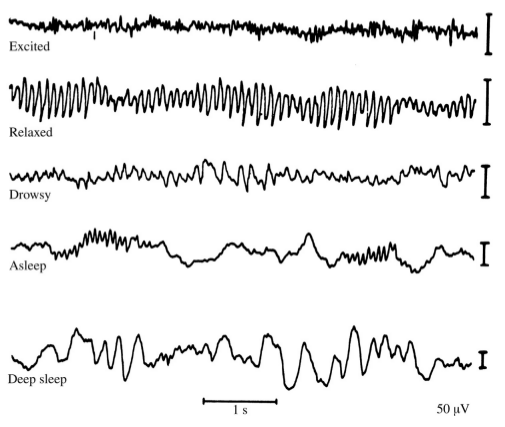
\includegraphics[width=0.7\linewidth]{figura_7.png} 
\caption{Los cambios en el EEG que ocurren durante el sue\~no en un sujeto.
Las marcas de calibraci\'on corresponden a 50 mV.
%H. Jasper, ‘‘Electrocephalography.’’ In Epilepsy and Cerebral Localization, W.
%G. Penfield and T. C. Erickson (eds.). Springfield, IL: Charles C. Thomas,
%1941.)
[Estos gr\'aficos ser\'an redibujados]
}
\label{ritmosEEG}
\end{figure}

%%%%%%%%%%%%%%%%%%%%%%%%%%%%%%%%%%%%%%%%%%%%%%%%%%%%%%%%%%%%%%%%%%%%%%%%%%%%%%%%%%%%%%%%%%%%%%%%%%%

\subsection{Etapas del sue\~no}

El sue\~no normal se divide en dos etapas: sue\~no  MOR (fase R)
%\footnote{Tambi\'en conocido como
%REM (Rapid-eyemovement)} (movimiento-ocular-r\'apido) 
y sue\~o no-MOR (fase N), los cuales se diferencian 
fundamentalmente por sus rasgos electroencefalogr\'aficos y una serie de caracter\'isticas 
fisiol\'ogicas --de los cuales surgen sus nombres.
Cabe mencionar que
la nomenclatura acerca de las fases del sue\~no ha sido 
recientemente modificada por la Academia Americana de Medicina del Sueño en 2007, 
de modo que en este trabajo se usar\'an ambas nomenclaturas siempre que sea posible, por fines
de compatibilidad con la terminolog\'ia usual.

%Una herramienta tecnol\'ogica que ha sido de vital importancia para el estudio de la fisiolog\'ia 
%del sue\~no es el electroencefalograma (EEG). De forma muy simplificada, el EEG es el la 
%representaci\'on gr\'afica y digital de las oscilaciones que muestra la actividad el\'ectrica 
%del cerebro, al ser registrada mediante electrodos colocados encima de la piel cabelluda en 
%distintas regiones de la cabeza \cite{Hita14}.

%El sue\~no MOR se caracteriza por la presencia de ondas de bajo voltaje y alta frecuencia en el 
%EEG, aton\'ia muscular y movimientos oculares r\'apidos, adem\'as es donde se presentan 
%la mayor\'ia de los sue\~nos. 
%El sue\~no no-MOR se compone de cuatro fases, 1 y 2, que son de sue\~no ligero, y 3 y 4 de 
%sue\~no profundo, las mismas que transcurren de manera secuencial desde la primera hasta la 
%cuarta fase, que es la fase reparadora del sue\~no, aquella que produce en la persona la 
%sensaci\'on de haber descansado cuando se levanta 13,22,43.

%Las características de las fases del sueño no-MOR incluyen cuatro etapas, la primera que 
%corresponde a la transición de la vigilia al sueño; la etapa 2 es la intermedia (mayor porcentaje 
%del tiempo de sueño) y en el EEG aparecen husos de sueño y los complejos K. La etapa 3 es la del 
%sueño relativamente profundo, representado en el electroencefalograma por ondas lentas de gran 
%amplitud, y la etapa 4o de sueño profundo con más del 50\% de ondas lentas de gran amplitud13.

%Durante el estado de alerta, mientras se mantienen los ojos cerrados, en el EEG se observan 
%oscilaciones de la actividad eléctrica que suelen encontrarse entre 8-13 ciclos por segundo (Hz), 
%principalmente a nivel de las regiones occipitales (ritmo alfa). Durante el sueño ocurren cambios 
%característicos de la actividad eléctrica cerebral que son la base para dividir el sueño en varias 
%fases. Como ya se mencionó, el sueño suele dividirse en dos grandes fases que, de forma normal, 
%ocurren siempre en la misma sucesión: todo episodio de sueño comienza con el llamado sueño sin 
%movimientos oculares rápidos (No MOR), que tiene varias fases, y después pasa al sueño con 
%movimientos oculares rápidos (MOR). 

%%%%%%%%%%%%%%%%%%%%%%%%%%%%%%%%%%%%%%%%%%%%%%%%%%%%%%%%%%%%%%%%%%%%%%%%%%%%%%%%%%%%%%%%%%%%%%%%%%%

\subsubsection{Sueño no-MOR (N)}

\begin{description}
\item[Fase 1 (N1)] Corresponde con la somnolencia o el inicio del sue\~no ligero, en ella es muy 
f\'acil despertarse. La actividad muscular disminuye paulatinamente y pueden observarse algunas 
breves sacudidas musculares s\'ubitas que a veces coinciden con una sensación de ca\'ida 
(mioclon\'ias h\'ipnicas). En el EEG se observa actividad de frecuencias mezcladas, pero de bajo 
voltaje y algunas ondas agudas (ondas agudas del v\'ertex). 

\item[Fase 2 (N2)] En el EEG se caracteriza por que aparecen patrones espec\'ificos de actividad 
cerebral llamados \textbf{husos de sue\~no} y \textbf{complejos K}. F\'isicamente la 
temperatura, la frecuencia cardiaca y respiratoria comienzan a disminuir paulatinamente. 

\item[Fases 3 y 4 (N3)] Sue\~no de ondas lentas, es la fase de sue\~no no-MOR m\'as profunda, 
y en el EEG se observa actividad de frecuencia muy lenta (< 2 Hz).
\end{description}

%%%%%%%%%%%%%%%%%%%%%%%%%%%%%%%%%%%%%%%%%%%%%%%%%%%%%%%%%%%%%%%%%%%%%%%%%%%%%%%%%%%%%%%%%%%%%%%%%%%

\subsubsection{Sueño MOR (R)}

Se caracteriza por la presencia de movimientos oculares r\'apidos. F\'isicamente el tono de todos 
los m\'usculos disminuye (con excepción de los m\'usculos respiratorios y los esf\'interes vesical 
y anal), as\'i mismo la frecuencia cardiaca y respiratoria se vuelve irregular.%,
%e incluso puede 
%incrementarse y 
%existe erección espontánea del pene o del clítoris. 
Durante el sue\~no MOR se producen la mayor\'ia de las enso\~naciones (lo que conocemos 
coloquialmente como sue\~nos), y la mayor\'ia de los pacientes que despiertan durante esta fase 
suelen recordar v\'ividamente el contenido de sus enso\~naciones \cite{Chokroverty09}.

%Por otro lado, las necesidades de sueño son muy variables según la edad y las circunstancias 
%individuales 43,54:
%Un niño recién nacido duerme casi todo el día, con una proporción próxima al 50\% del denominado 
%sueño «activo», que es el equivalente del sueño MOR. A lo largo de la lactancia los períodos de 
%vigilia son progresivamente más prolongados y se consolida el sueño de la noche; además, la 
%proporción de sueño MOR desciende al 25-30 \%, que se mantendrá durante toda la vida. Entre el 1er 
%y 3er año de vida el niño ya sólo duerme una o dos siestas. Entre los 4 y 5 años y la adolescencia 
%los niños son hipervigilantes, muy pocos duermen siesta, pero tienen un sueño nocturno de 9-10 
%horas bien estructurado en 5 ciclos o más. Por lo que se refiere a los individuos jóvenes, en 
%ellos reaparece en muchos casos la necesidad fisiológica de una siesta a mitad del día43,55.

%%%%%%%%%%%%%%%%%%%%%%%

%La necesidad de sue\~no en un adulto puede oscilar entre 5 y 9 horas. Asimismo, var\'ia 
%notablemente el horario de sueño entre noct\'ambulos y madrugadores. En \'epocas de mucha actividad 
%intelectual o de crecimiento o durante los meses del embarazo, puede aumentar la necesidad de 
%sue\~no, mientras que el estr\'es, la ansiedad o el ejercicio f\'isico practicado por la tarde 
%pueden reducir la cantidad de sue\~no. 

%%%%%%%%%%%%%%%%%%%%%%%

%Los estudios efectuados en individuos aislados de influencias exteriores han mostrado que la 
%tendencia fisiológica general es a retrasar ligeramente la fase de sueño con respecto al ciclo 
%convencional de 24 horas y a dormir una corta siesta “de mediodía” 43,56. 
Un adulto j\'oven pasa aproximadamente entre 70--100 min en el sue\~no no-MOR para despu\'es entrar 
al sue\~no MOR, el cual puede durar entre 5--30 min; este ciclo se repite cada hora y media.
%durante toda la noche de sue\~no. 
A lo largo de la noche pueden presentarse normalmente entre 4 y 6 ciclos de 
sue\~no MOR.
En los ancianos se va fragmentando el sue\~no nocturno con frecuentes episodios de despertar, y se 
reduce mucho el porcentaje de sue\~no en fase 4 y no tanto el de sue\~no MOR, que se mantiene 
m\'as constante.% a lo largo de la vida. 
%Las personas de edad avanzada tienen tendencia a aumentar el tiempo de permanencia en la cama. 
%Muchas de ellas dormitan 
Adicionalmente, muchos adultos mayores dormitan
%f\'acilmente 
durante el d\'ia varias siestas cortas\cite{CarrilloMora}.

%%%%%%%%%%%%%%%%%%%%%%%%%%%%%%%%%%%%%%%%%%%%%%%%%%%%%%%%%%%%%%%%%%%%%%%%%%%%%%%%%%%%%%%%%%%%%%%%%%%

%\subsection{Alteraciones del ciclo vigilia-sueño}
%
%La relevancia que tiene el sueño para para la supervivencia de un individuo es la cantidad de horas que este duerme a lo largo de su vida, mismas que depende fundamentalmente de sus necesidades fisiológicas y de las demandas del ambiente al que está expuesto 4,57
% En el caso de los humanos, es posible establecer una clasificación de patrones de sueño en función de su duración (corta, intermedia y larga) 4. Las personas que muestran un patrón de sueño intermedio, es decir, duración aproximada de entre 7-8 horas, presentan un mejor estado de salud a lo largo de su vida, comparado con los individuos de duración de sueño corta o excesivamente larga que frecuentemente tienen de problemas de salud y/o laborales 42,45,46 . 
 
%La estabilidad del sue\~no nocturno es otro factor a tener en cuenta debido a que es razonable 
%pensar que un sue\~no muy fragmentado no cumplir\'a con sus funciones fisiol\'ogicas de igual forma 
%que un patr\'on de sue\~no estable a lo largo de la noche.

%%%%%%%%%%%%%%%%
%%%%%%%%%%%%%%%%
%
%Los adultos mayores informan que duermen menos durante la noche, y se acuestan y se despiertan 
%m\'as temprano de lo habitual. Adem\'as, tardan m\'as tiempo en conciliar el sue\~no, se 
%despiertan con m\'as frecuencia durante la noche y la duraci\'on de estos despertares es 
%m\'as prolongada 58,59.
%
%%%%%%%%%%%%%%%%
%%%%%%%%%%%%%%%%

%La disminución del tiempo de sueño asociada a un incremento de la somnolencia diurna incide negativamente en la función cerebral del día siguiente 60
%Por otro lado, existen diversas formas de pérdida de sueño13,25,46: a) la privación de sueño, que quiere decir la suspensión total del sueño por un periodo ($>$ 24 h), b) la restricción del sueño, que significa una disminución del tiempo habitual de sueño, generalmente de forma crónica, y c) la fragmentación del sueño, que significa la interrupción repetida (despertares) de la continuidad del sueño14. Todos estos tipos de alteraciones del sueño han demostrado afectar distintas funciones cognitivas y variedades de memoria en mayor o menor grado.

%Las alteraciones de sueño específicamente en personas mayores se han asociado con la presencia de enfermedades crónicas, problemas físicos y de salud mental 3

%%%%%%%%%%%%%%%%%%%%%%%%%%%%%%%%%%%%%%%%%%%%%%%%%%%%%%%%%%%%%%%%%%%%%%%%%%%%%%%%%%%%%%%%%%%%%%%%%%%
%%%%%%%%%%%%%%%%%%%%%%%%%%%%%%%%%%%%%%%%%%%%%%%%%%%%%%%%%%%%%%%%%%%%%%%%%%%%%%%%%%%%%%%%%%%%%%%%%%%